\section{oosalizer/parser.h-Dateireferenz}
\label{parser_8h}\index{oosalizer/parser.h@{oosalizer/parser.h}}


Dieser Graph zeigt, welche Datei direkt oder indirekt diese Datei enth\"{a}lt:\begin{figure}[H]
\begin{center}
\leavevmode
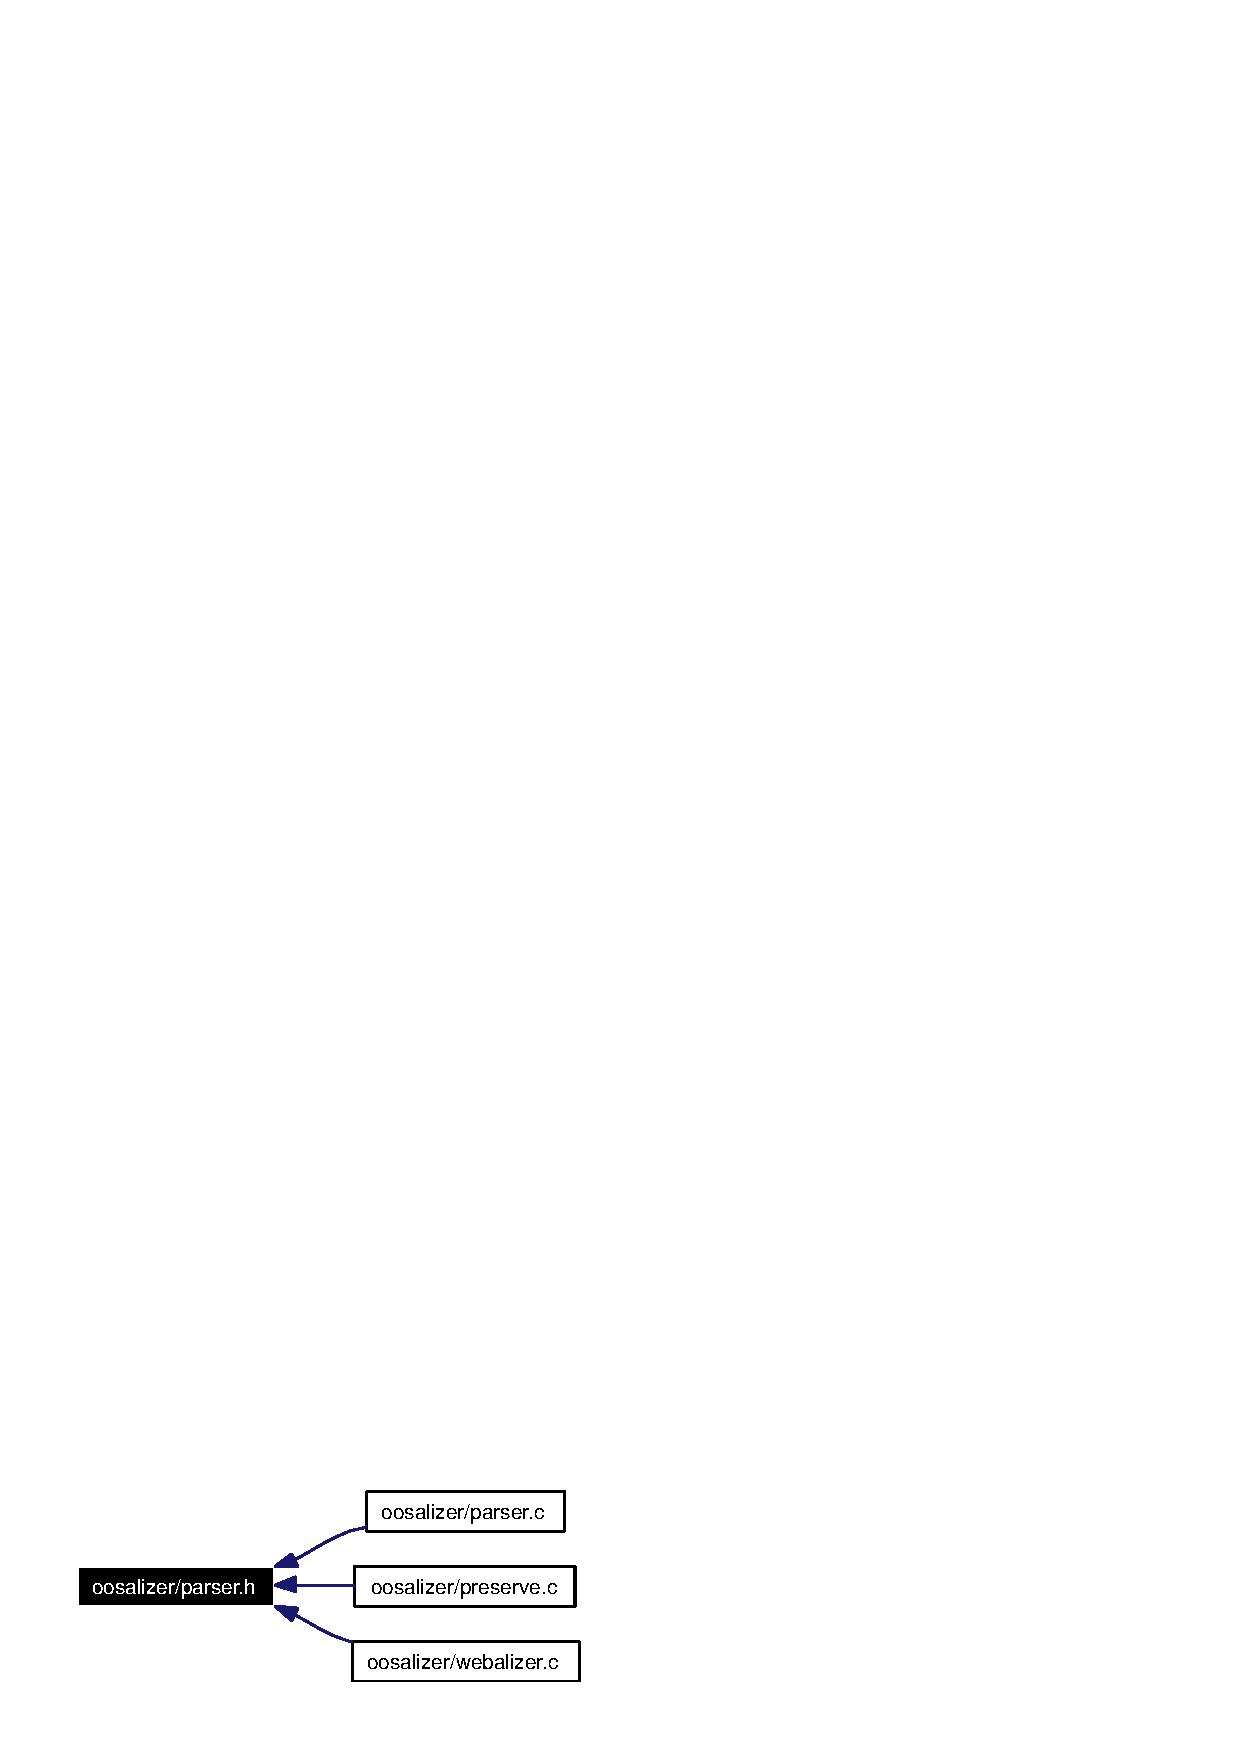
\includegraphics[width=139pt]{parser_8h__dep__incl}
\end{center}
\end{figure}
\subsection*{Funktionen}
\begin{CompactItemize}
\item 
int {\bf parse\_\-record} (char $\ast$)
\end{CompactItemize}


\subsection{Dokumentation der Funktionen}
\index{parser.h@{parser.h}!parse_record@{parse\_\-record}}
\index{parse_record@{parse\_\-record}!parser.h@{parser.h}}
\subsubsection{\setlength{\rightskip}{0pt plus 5cm}int parse\_\-record (char $\ast$)}\label{parser_8h_2e298d5e806fc4936bf6b142c0913a31}




Definiert in Zeile 101 der Datei parser.c.

Benutzt LOG\_\-CLF, LOG\_\-FTP, log\_\-rec, LOG\_\-SQUID, log\_\-type, parse\_\-record\_\-ftp(), parse\_\-record\_\-squid() und parse\_\-record\_\-web().